\documentclass[border=3pt]{standalone}
% Preâmbulo compartilhado pelos diagramas TikZ da aula 8 de IHR (Métodos de Pesquisa)
\usepackage[T1]{fontenc}
\usepackage[utf8]{inputenc}
\usepackage{lmodern}
\usepackage{amsmath}
\usepackage{xcolor}
\usepackage{tikz}
\usetikzlibrary{arrows.meta,angles,quotes,decorations.pathmorphing,decorations.pathreplacing,calc,
                positioning,shapes.geometric,shapes.misc,backgrounds,fit,
                math}

% Paleta (mesma dos SVGs originais)
% Paleta da disciplina de IHR: acento azul (#1A6FB5), cor de destaque do tema.
% (o nome "dblue" é mantido para não alterar todos os diagramas)
\definecolor{dblue}{HTML}{1A6FB5}
\definecolor{dorange}{HTML}{B3541E}
\definecolor{dgreen}{HTML}{4A7C59}
\definecolor{dred}{HTML}{9C4B4B}
\definecolor{dcream}{HTML}{F4F1EA}
\definecolor{dshade}{HTML}{DDD7C9}

% Função gaussiana (não normalizada por padrão de escala visual)
\pgfmathdeclarefunction{gauss}{3}{%
  \pgfmathparse{1/(#3*sqrt(2*pi))*exp(-((#1-#2)^2)/(2*#3^2))}%
}

% Estilos comuns (prefixo d... para não colidir com chaves internas do pgf)
\tikzset{
  >={Stealth[length=2mm]},
  dguide/.style={gray!55, dashed, line width=0.4pt},
  daxis/.style={gray!60, line width=0.7pt, ->},
  dbody/.style={fill=black!3, draw=black!80, line width=1pt},
  dacc/.style={draw=dblue, line width=1pt},
  dlbl/.style={black!55, font=\small},
  dsub/.style={black!45, font=\footnotesize},
  dstate/.style={circle, draw=black!80, fill=dcream, line width=1pt,
                 minimum size=17mm, font=\large, inner sep=1pt},
  dobs/.style={circle, draw=black!80, fill=dshade, line width=1pt,
               minimum size=14mm, font=\large, inner sep=1pt},
  dbox/.style={rounded corners=2pt, draw=black!80, fill=dcream, line width=1pt,
               align=center, inner sep=6pt},
  dop/.style={circle, draw=black!80, fill=white, line width=1pt,
              minimum size=6mm, inner sep=0pt, font=\small},
  dtrans/.style={->, dblue, line width=1pt},
  dmeas/.style={->, dorange, line width=1pt},
  dcurve/.style={line width=1pt, dblue},
  dcurveb/.style={line width=1.4pt, dorange},
}

\begin{document}
\hyphenpenalty=10000 \exhyphenpenalty=10000 \tolerance=9999 \emergencystretch=3em
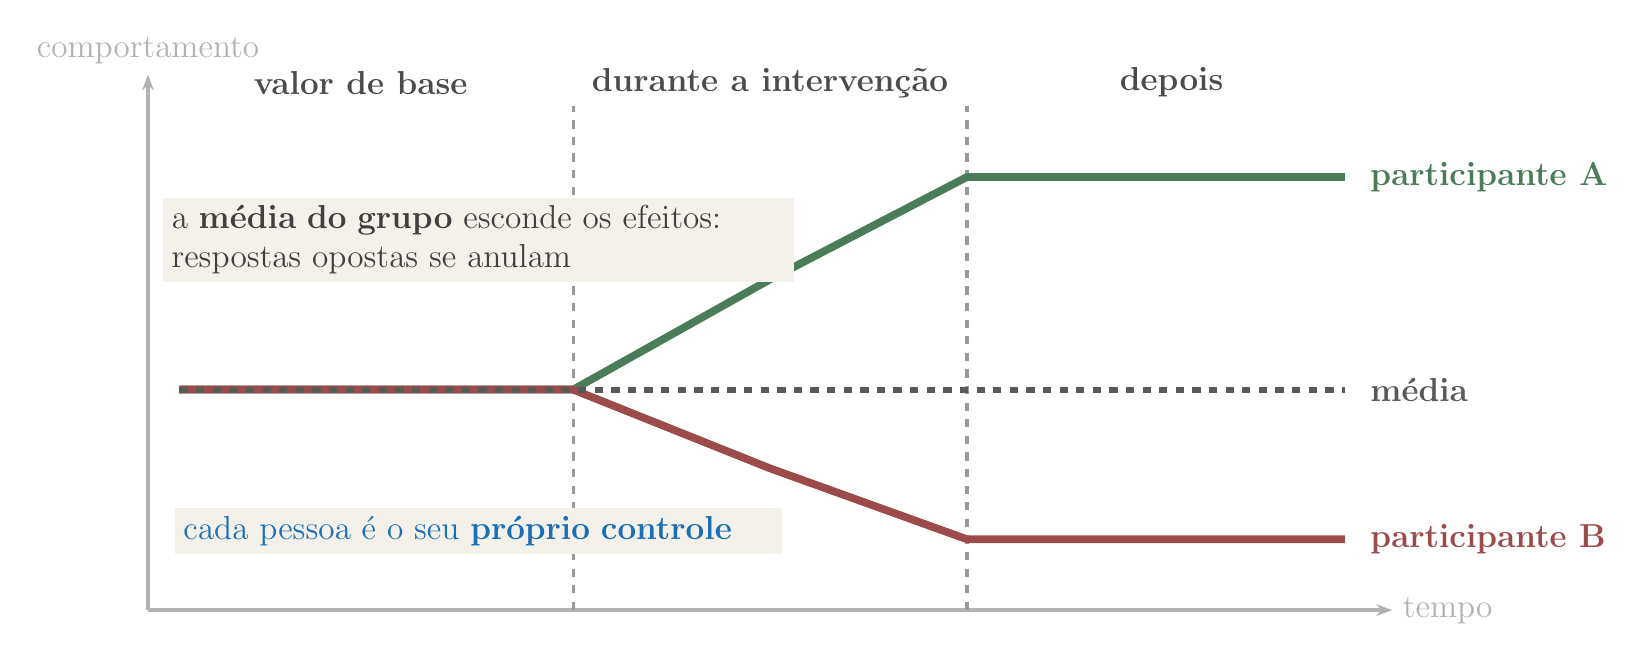
\begin{tikzpicture}[x=1cm,y=1cm]
  \draw[daxis, line width=1.2pt] (1.0,0.8) -- (16.8,0.8) node[right, font=\large] {tempo};
  \draw[daxis, line width=1.2pt] (1.0,0.8) -- (1.0,7.6) node[above, font=\large] {comportamento};
  \draw[black!40, dashed, line width=1.2pt] (6.4,0.8) -- (6.4,7.2);
  \draw[black!40, dashed, line width=1.2pt] (11.4,0.8) -- (11.4,7.2);
  \node[font=\large\bfseries, black!70] at (3.7,7.5) {valor de base};
  \node[font=\large\bfseries, black!70] at (8.9,7.5) {durante a intervenção};
  \node[font=\large\bfseries, black!70] at (14.0,7.5) {depois};
  \draw[dgreen, line width=2.8pt, line join=round] (1.4,3.6) -- (6.4,3.6) -- (8.9,5.0) -- (11.4,6.3) -- (16.2,6.3);
  \draw[dred, line width=2.8pt, line join=round] (1.4,3.6) -- (6.4,3.6) -- (8.9,2.6) -- (11.4,1.7) -- (16.2,1.7);
  \draw[black!65, dashed, line width=2.2pt] (1.4,3.6) -- (16.2,3.6);
  \node[font=\large\bfseries, dgreen, anchor=west] at (16.4,6.3) {participante A};
  \node[font=\large\bfseries, dred, anchor=west] at (16.4,1.7) {participante B};
  \node[font=\large\bfseries, black!65, anchor=west] at (16.4,3.6) {média};
  \node[font=\large, black!75, text width=7.8cm, align=left, fill=dcream, inner sep=3pt] at (5.2,5.5) {a \textbf{média do grupo} esconde os efeitos: respostas opostas se anulam};
  \node[font=\large, dblue, text width=7.5cm, align=left, fill=dcream, inner sep=3pt] at (5.2,1.8) {cada pessoa é o seu \textbf{próprio controle}};
\end{tikzpicture}
\end{document}
